\chapter{Implementation}



\section{LSP server}

Our tool is integrated into IDEs via the Language server protocol. The goal is to give
users of the tool a overview of all clones as they appear in source-code

The following user-stories shows how interaction with the LSP server works.

\begin{itemize}
	\item A programmer wants to see code clones for a file in their project, the
	      programmer opens the file in their IDE and is displayed diagnostics in the code
	      wherever there are detected clones. The matching code clones are not necessarily
	      in the same file.

	\item A programmer wants to see all code clones for the current project. The
	      programmer opens the IDEs diagnostic view and will see all code clones detected
	      as diagnostics there. The diagnostic will contain information like where the clone
	      exists, and where the matching clone(s) are.

	\item A programmer wants to jump to the corresponding match of a code clone in their
	      editor. The programmer moves their cursor to the diagnostic and will see a list of
	      the matching code clones. The programmer will select the wanted code clone which
	      will move the cursor to the file and location of the selected code clone.
          Alternatively, a code-action can be invoked to navigate, if the client does not
          implement the ''DiagnosticRelatedInformation`` interface.

      \item A programmer wants to remove a set of clones by applying the
          ``extract-method'' refactoring. The programmer performs the necessary
          refactorings, saves the file and will get quick feedback whether the
          clones are now gone.
\end{itemize}

% TODO redo this figure
\begin{figure}
	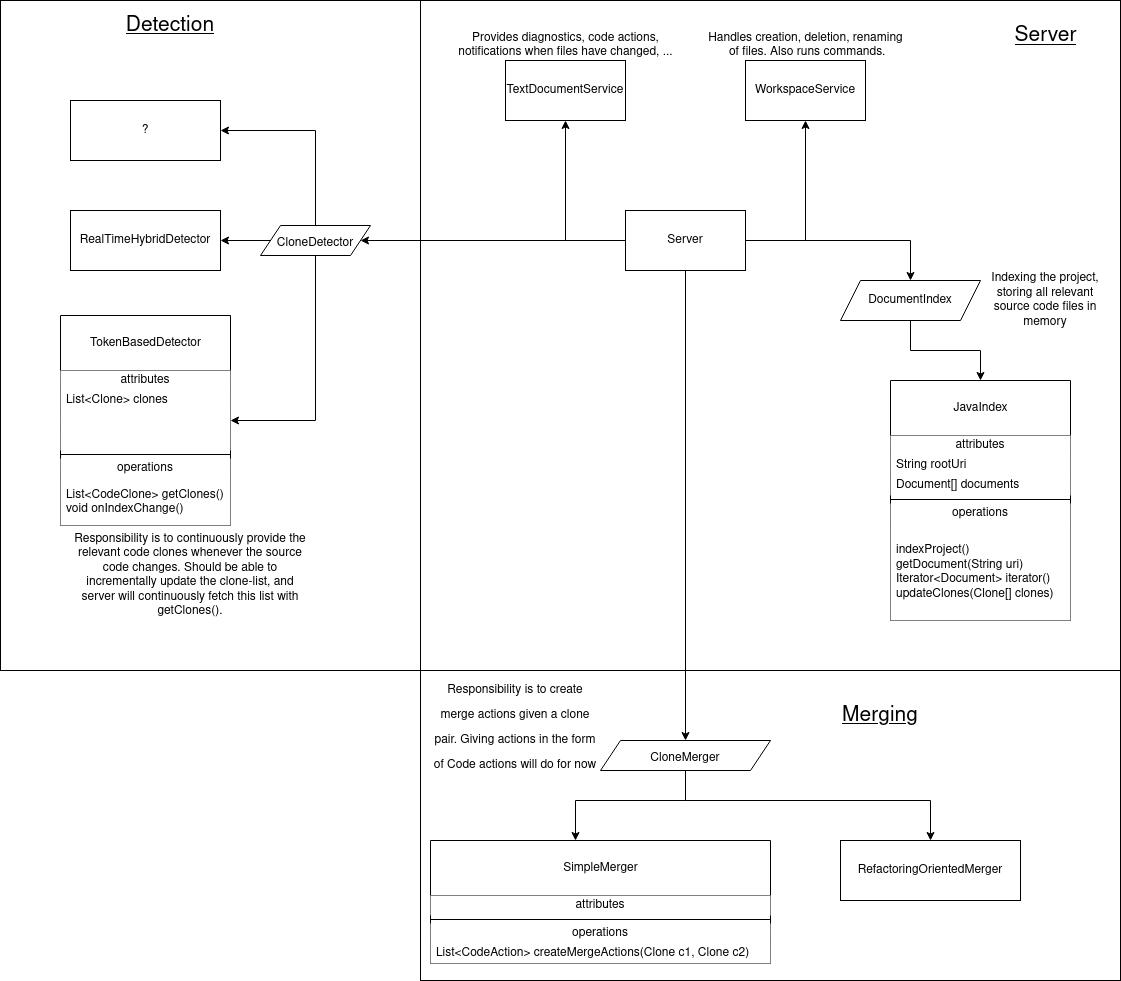
\includegraphics[width=\textwidth]{images/ToolArchitecture.png}
	\caption{Tool architecture}
	\label{fig:architecture}
\end{figure}


Figure \ref{fig:architecture} shows the architecture of the tool. The server communicates
with the IDE and delegates the work of managing clones to the detection engine and the
merge engine. The tool also stores an index of all source code files in the current project.

\subsection{Document index}

\subsection{Displaying and interacting with clones}

\section{Detection algorithm}


\subsection{Fragment selection}

\subsection{Fingerprinting}

\subsection{Suffix array construction}

\subsection{Clone detection}

\subsection{Incremental updates}
